\documentclass[conference]{IEEEtran}
\IEEEoverridecommandlockouts
% The preceding line is only needed to identify funding in the first footnote. If that is unneeded, please comment it out.
\usepackage{cite}
\usepackage{amsmath,amssymb,amsfonts,dsfont}
\usepackage{algorithmic}
\usepackage{graphicx}
\usepackage{textcomp}
\usepackage{xcolor}
\usepackage{xr}
\def\BibTeX{{\rm B\kern-.05em{\sc i\kern-.025em b}\kern-.08em
    T\kern-.1667em\lower.7ex\hbox{E}\kern-.125emX}}
\begin{document}

\title{Sharing and Binding for General Circuits\\
{\footnotesize }
\thanks{Identify applicable funding agency here. If none, delete this.}
}

\author{\IEEEauthorblockN{1\textsuperscript{st} Sheikh Muhammad Adib Bin Sh Abu Bakar}
\IEEEauthorblockA{\textit{Hochshule Hamm-Lippstadt} \\
\textit{B.Eng. Electronic Engineering}\\
Lippstadt, Germany \\
sheikh-muhammad-adib.bin-sh-abu-bakar@stud.hshl.de}

}

\maketitle

\begin{abstract}

Producing an optimum circuit is the dream of every circuit designer. A circuit can be evaluated through its used area and performance. Those aspects are designer concern to be optimized that can be done only during architectural synthesis or known as high level synthesis. Resource sharing and binding are very important process in circuit optimization. In this paper, sharing and binding will be discussed mainly for general circuit. This includes a sample model circuit to ease the explanation process and the method used for sharing and binding. After that, the strategies for optimization that use all those methods will be explored.

\end{abstract}

\begin{IEEEkeywords}
sharing, binding, general circuit, optimization
\end{IEEEkeywords}
\begin{IEEEkeywords}
sharing, binding, general circuit, optimization
\end{IEEEkeywords}


\input{Introduction.tex}
\section{Basic Concept}


\subsection{Clique Covering and Clique Panitioning}

Clique partitioning and clique covering are closely related. A clique partition is a disjoint clique cover. A clique cover that is not disjoint can be made disjoint by selecting a set of disjoint cliques each contained in a corresponding clique of the cover. Finding a clique cover, or partition, with bounded cardinality is an intractable problem [??]. 
A partition into cliques can be obtained by coloring the complement of the graph. Indeed each clique identifies a set of pairwise adjacent vertices, which are not adjacent in the graph complement, and thus can be colored with the same color. Therefore the clique cover number of a graph corresponds to the chromatic number of its complement. As a result, heuristic and exact algorithms for coloring can be applied to the search of minimum-cardinality clique partitions. 

\subsection{Data Flow Sequencing Graph}

evel are in terms of tasks (or operations) and their dependencies. Tasks may be No Operations (NOPs), i.e., fake operations that execute instantaneously with no side effect. Dependencies arise from several reasons. A first reason is availability of data. When an input to an operation is the result of another operation, the former operation depends on the latter. A second reason is serialization constraints in the specification. A task may have to follow a second one regardless of data dependency. A simple example is provided by the two following operations: loading data on a bus and raising a flag. The circuit model may require that the flag is raised after the data are loaded. Last, dependencies may arise because two tasks share the same resource that can service one task at a time. Thus one task has to perform before the other. Note, though, that, in general, dependencies due to resource sharing are not part of the original circuit specification, because the way in which resources are exploited is related to the circuit implementation. 

Data-flow graphs represent operations and data dependencies. Let the number of operations be n,,. A data-flow graph $ G_{d}(V, E) $ is a directed graph whose vertex set $ V = \{v_{i}; i = 1,2,...,n_{ops}) $ is in one-to-one correspondence with the set of tasks. We assume here that operations require one or more operands and yield one or more results (e.g., an addition with two addends yielding a result and an overflow flag). The directed edge set $ E= \{(v_{i},v_{j}); i,j = 1,2,...,n_{ops}) $  is in correspondence with the transfer of data from an operation to another one. Data-flow graphs can be extended by adding other types of depend

\subsection{Resources Type}

Resources implement different types of functions in hardware. They can be broadly classified as follows: 

\begin{itemize}
\item Functional resources process data. They implement arithmetic or logic functions and can be grouped into two subclasses: 

\begin{itemize}
\item  Primitive resources are subcircuits that are designed carefully once and often used. Examples are arithmetic units and some standard logic functions, such as encoders and decoders. Primitive resources can be stored in libraries. Each resource is fully characterized by its area and performance parameters. 
\item  Application-specific resources are subcircuits that solve a particular subtask. 
\end{itemize}

\item An example is a subcircuit servicing a particular intempt of a processor. In general such resources are the implementation of other HDL models. When synthesizing hierarchical sequencing graph models bottom up, the implementation of the entities at lower levels of the hierarchy can be viewed as resources. 


\item Memory resources store data. Examples are registers and read-only and read-write memory arrays. Requirement for storage resources are implicit in the sequencing graph model. In some cases, access to memory arrays is modeled as transfer of data across circuit ports. 


\item Interface resources support data transfer. Interface resources include busses that may he used as a major means of communication inside a data path. External interface resources are UO pads and interfacing circuits. 

\end{itemize}

\subsection{Constraint Definition}

Constraints in architectural synthesis can be classified into two major groups: interface constraints and implementatron constraints. 
Interface constraints are additional specifications to ensure that the circuit can be embedded in a given environment. They relate to the format and timing of the I/O data transfers. The data format is often specified by the interface of the model. The timing separation of UO operations can be specified by timing constraints that can ensure that a synchronous I/O operation follows/precedes another one by a prescribed number of cycles in a given interval. Timing constraints can also specify data rates for pipelined systems. Implementation constraints reflect the desire of the designer to achieve a structure with some properties. Examples are area constraints and performance constraints, e.g., cycle-time and/or latency bounds. 
A different kind of implementation constraint is a resource b~nding constraint. In this case, a particular operation is required to be implemented by a given resource. These constraints are motivated by the designer's previous knowledge, or intuition, that one particular choice is the best and that other choices do not need investigation. Architectural synthesis with resource binding constraints is often referred to as synthesis from partial structure [??]. Design systems that support such a feature allow a designer to specify a circuit in a wide spectrum of ways, ranging from a full behavioral model to a structural one. This modeling capability may be useful to leverage previously designed components. 






\input{Problem.tex}
\section{Resource Sharing and Binding Analysis}

As explain before two or more operation can be bound to the same resource. Before we bond them together we need to ensure that they are \textit{compatible}. Two conditions that the operations should met in order to be \textit{compatible} :

\begin{itemize}
\item The operations is not concurrent.
\item The operations can be implemented by resources of the same type.
\end{itemize}

So, $ E+\{(v_{i},v_{j})|\tau(v_{i}=v_{j} $ and $ ((t_{i}=d_{i} \leq t_{j}) $ or $ t_{j}=d{j} \leq t_{i})),i,j=1,...,n_{ops}\}$ %

In general, the compatibility can be analyzed using compatibility graph, conflict graph. The sample problem that I will use for the explanation is from figure \ref{fig:Scheduled_sequencing_graph}


\subsection{Compatibility Graph}


$G_{+}(V,E)$ is a graph whose vertex set  $  V = \{v_{i}, i = 1,2,..., n_{ops}\} $ is in one to one correspondence with the operation and whose edge set $ E = \{\{v_{i},v_{j} i,j = 1,2,...,n_{ops}\}$ denotes the compatible operation pairs \cite{b1}. 

Means that the number of disjoint component in the graph has atleast the same number with the resource types. An optimum resources sharing is one that minimizes the number of required resources instance \cite{b1}.

According to \cite{b1} - A group of mutually compatible operations corresponds to a subset of vertices that are all mutually connected by edges, i.e., to a clique. Therefore a minimal set of mutually compatible operations is represented by a maximal clique in the compatibility graph. Since we can associate a resource instance to each clique, the problem is equivalent to partitioning the graph into a minimum number of cliques. Such a number is the clique cover number of $G_{+}(V,E)  $, denoted by $\kappa(G_{+}(V,E)) $

Figure \ref{fig:Compatibility_graph} is an example of compatibility graph base on sequencing graph in figure\ref{Scheduled_sequencing_graph}. We can see that $\{v_{2},v_{6}\}  $ and $\{v_{10},v_{11}\} $ are examples of compatible operation.  Examples of cliques are the subgraphs induced by $\{v_{1},v_{3},v_{7}\}  $,$\{ v_{2},v_{6},v_{8}\} $,$\{ v_{4},v_{5}, v_{10}, v_{11}\}$ $ \{v_{9}\} $. So the clique cover number $ \kappa $ of the graph is 4, corresponding to two multipliers and two ALUs. Edges of the cliques are emboldened in Figure \ref{fig:Compatibility_graph}.


\ref{fig:Compatibility_graph}
\begin{figure}[h]
    \centering
    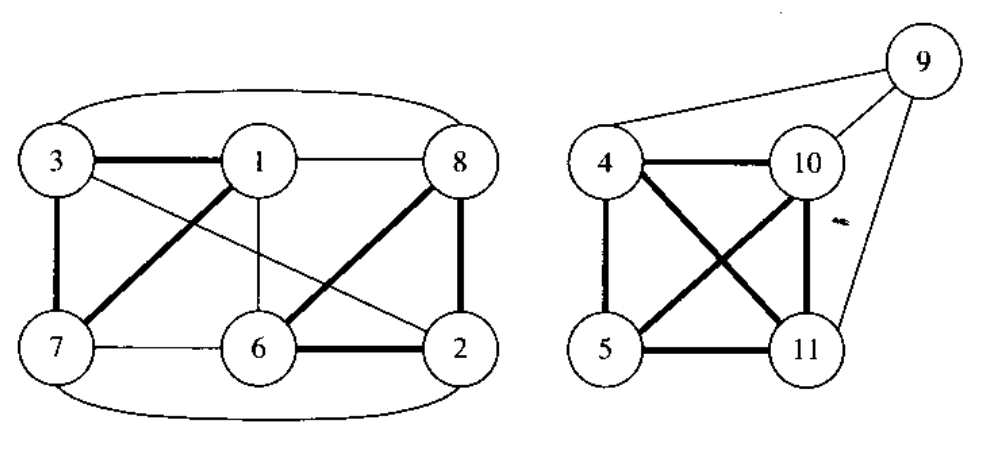
\includegraphics[width=0.5\textwidth]{Compatibility_graph}
    \caption{ Compatibility graph \cite{b1}}
    \label{fig:Compatibility_graph}
\end{figure}


\subsection{Conflict Graph}
$G_{-}(V,E)  $,  is a graph whose vertex set $  V = \{v_{i}, i = 1,2,..., n_{ops}\} $ is in one-to-one correspondence with the operations and whose edge set $ E = \{\{v_{i},v_{j} i,j = 1,2,...,n_{ops}\}$ denotes the conflicting operation pairs \cite{b1}. 

$G_{-}(V,E) $ is the compliment of $G_{+}(V,E)  $ because A set of mutually compatible operations corresponds to a subset of vertices that are not connected by edges, also called the independent set $G_{-}(V,E)  $. A proper vertex coloring of the conflict graph provides a solution to the sharing problem: each color corresponds to a resource instance. An optimum resource sharing corresponds to a vertex coloring with a minimum number of colors. Such a number is the chromatic number of G-(V, E) and is denoted by x(G-(V, E)). Note that 
\begin{center}
$\chi(G_{-}(V,E))  \Leftrightarrow \kappa(G_{+}(V,E)) $
\end{center}

Since operations with different types are always conflicting, it is convenient to consider the conflict graphs for each type independently. Such graphs are the complements of the corresponding compatibility subgraphs for operations of that type. The overall conflict graph can be obtained by adding edges joining any vertex pair with different types to the union of all partial conflict graphs. 

Consider again the scheduled sequencing graph of Figure \ref{Scheduled_sequencing_graph}. We show in Figure \ref{fig:Conflict_graphs_for_the_mtlltiplier_and_ALU_types} the conflict graphs for the multiplier and ALU types. Examples of independent sets are $\{v_{1},v_{3},v_{7}\}  $and$ v_{4},v_{5},v_{10},v_{11} $ among others. Each graph can he colored The clique partitioning and vertex coloring problems have been studied extensively. (See Sections 2.4.4 and 2.4.3.) Both problems are intractable for general graphs, and exact and heuristic solution methods have been proposed. According to the specific circuit type under consideration, the compatibility graph may be sparser than the conflict graph (or vice versa). In this case, clique partitioning (or vertex coloring) may be easier to solve. 


\ref{fig:Conflict_graphs_for_the_mtlltiplier_and_ALU_types}
\begin{figure}[h]
    \centering
    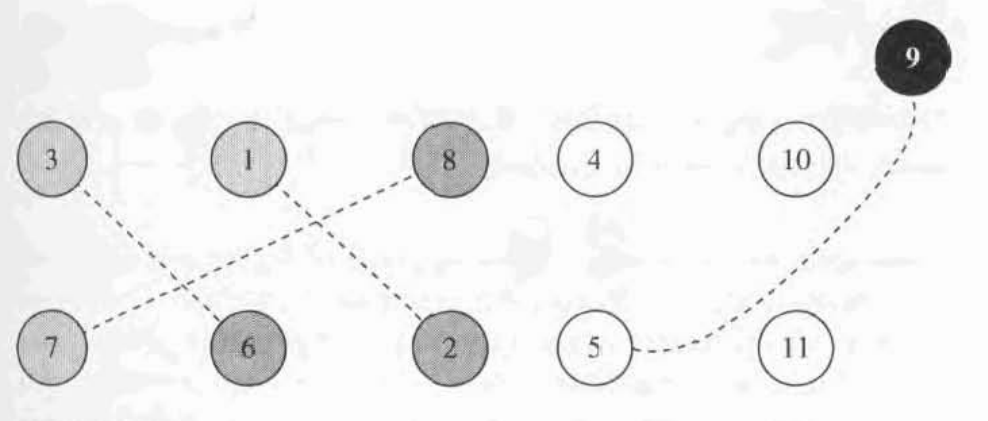
\includegraphics[width=0.5\textwidth]{Conflict_graphs_for_the_mtlltiplier_and_ALU_types}
    \caption{Conflict graphs for the mtlltiplier and ALU types.Conflict graphs for the mtlltiplier and ALU types. \cite{b1}}
    \label{fig:Conflict_graphs_for_the_mtlltiplier_and_ALU_types}
\end{figure}


In some particular cases, it is possible to exploit the structure of the sequencing graph to derive compatibility and conflict graphs with special properties that make the partitioning and coloring tractable. This will be considered in the following section.



\subsection{Conflict graph as an interval for non hierarchical graph}


Let us consider now the conflict graphs for each resource type. The execution intervals for each operation are $ \{[t_{i},t_{i}+d_{i}-1];i=1,2,...,n_{ops}\} $ and the edges of the conflict graphs denote intersections among intervals; hence they are interval graphs. The search for a minimum coloring of an interval graph can be achieved in polynomial time.  Usually, resource Sharing and binding is achieved by considering the conflict graphs for each type, because resources are assumed to have a single type. Thus, the overall conflict graph is of limited interest, even though it can be derived from the conflict graphs of each resource type in a straightforward way.

Consider again the scheduled sequencing graph of Figure \ref{Scheduled_sequencing_graph}, where all operations have unit execution delay. The set of intervals corresponding to the conflict graphs is shown in Figure \ref{Intervals_corresponding_to_the_conflict_grap}. Overlapping intervals correspond to edges in the conflict 
graph for each type. When considering the multiplier, the conflict edges are $ \{v_{1},v_{2}\} $,$ \{v_{3},v_{6}\} $ and $ \{v_{7},v_{8}\} $. When considering the ALU, the conflict edge is $ \{v_{5},v_{9}\} $.


\begin{figure}[h]
    \centering
    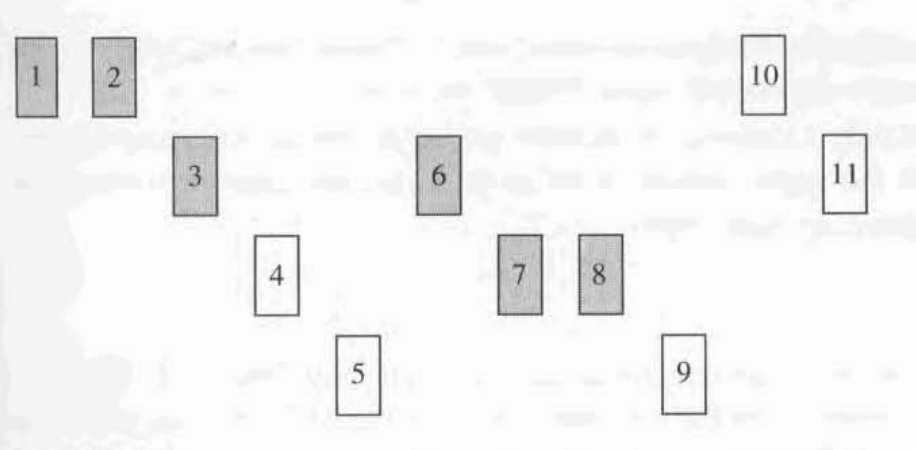
\includegraphics[width=0.5\textwidth]{Intervals_corresponding_to_the_conflict_grap}
    \caption{ Intervals corresponding to the conflict graph \cite{b1}}
    \label{fig:Intervals_corresponding_to_the_conflict_grap}
\end{figure}


\begin{figure}[h]
    \centering
    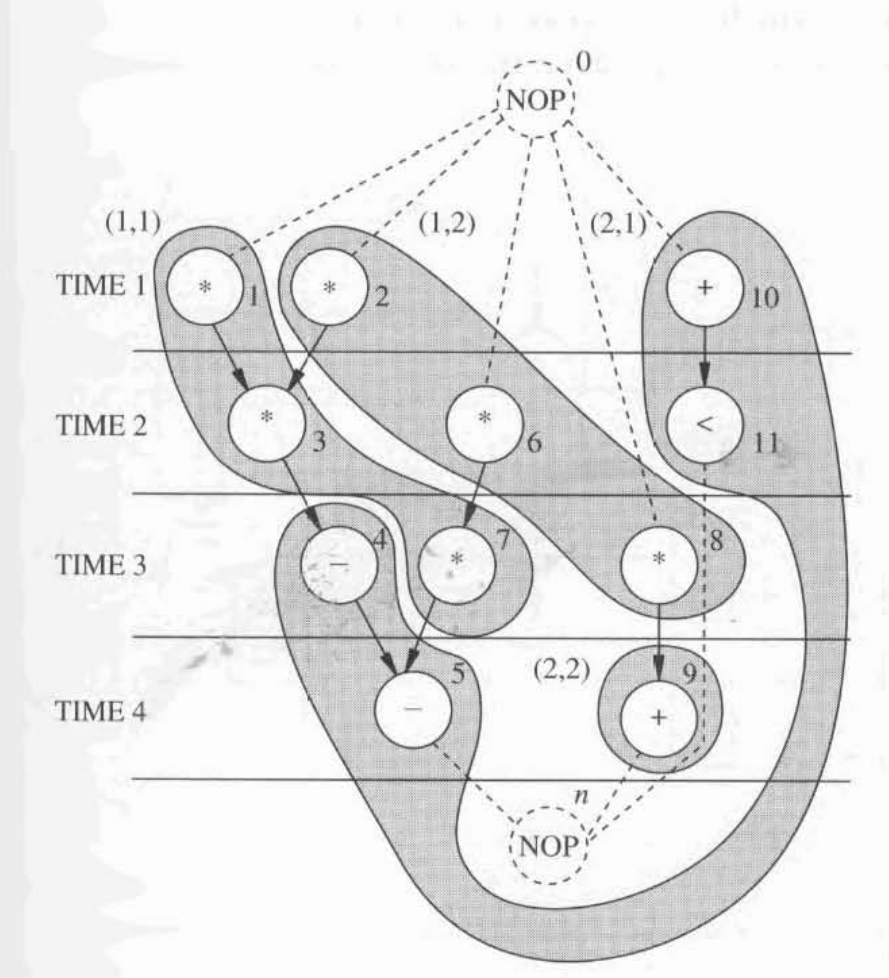
\includegraphics[width=0.5\textwidth]{Scheduled_an_bound_sequencing}
    \caption{ Scheduled and bound sequencing graph \cite{b1}}
    \label{fig:Scheduled_an_bound_sequencing}
\end{figure}

\subsection{Analysis using ILP model}

It is instructive to show that the binding problem can be formulated with an ILP model. For the sake of simplicity, we assume first that all operations and resources have the same type. We use a set of binary decision variables with two indices, $ B=\{b_{ir};i=1,2,...,n_{pos};r=1,2,...,a\} $, and a set of binary decision constants with two indices, $ X=\{x_{il};i=1,2,...,n_{pos};l=1,2,...,\lambda+1\} $, where $ a\leq n_{ops} $ is an upper bound on the number of resources to be used. We use the set notation for the variables in B, rather than a matrix notation, because we do not make use of matrix operations. The binary variable,$ b_{ir} $ is 1 only when operation $ v_{i} $ is bound to resource r, i.e., $ \beta(v_{i})=(1,r) $. The binary constant, $ x_{il} $ is 1 only when operation $ v_{i} $  starts in step 1 of the schedule, i.e., $ l = t{i} $. These values are known constants, because we consider scheduled sequencing graphs. 

Searching for a binding compatible with a given schedule (represented by X) and a resource bound a is equivalent to searching for a set of values of B satisfying 
the following constraints: 

\begin{equation}\label{a}
 \sum_{r=1}^{a} b_{ir} = 1, i=1,2,...,n_{ops} 
\end{equation}

\begin{equation}\label{b}
\sum_{i=1}^{n_{ops}} b_{ir}\sum_{m=l-d_{i}+1}^{l} x_{im} \leq 1, l=1,2,...,\lambda + 1, r=1,2,...,a 
\end{equation}

\begin{equation}\label{c}
b_{ir} \in \{0,1\}, 1 =1,2,...,n_{ops}, r=1,2,...,a
\end{equation}

Constraint \ref{a} states that each operation $ v_{i} $  should be assigned to one and only one resource. Constraint \ref{b} states that at most one operation can be executing, among 
those assigned to resource r, at any time step. Note that it suffices to require the variables in B to he non-negative integers to satisfy \ref{c}. Hence the problem can be formulated as an ILP and not necessarily as a ZOLP. 
This model can be easily extended to include multiple operation types. Nevertheless, the disjointness of the types makes it easier to formulate and solve as many independent binding problems as each type. 

Consider again the scheduled sequencing graph of Figure \ref{Scheduled_sequencing_graph}. The operations have two types (labeled 1 for the multiplier and 2 for the ALU) and unit execution delays. Therefore a feasible binding satisfies the constraints: 

\begin{center}

$ \sum_{r=1}^{a_{1}} b_{ir} = 1,\forall_{i} : \tau(v_{i})=1 $

$ \sum_{i=:\tau(v_{i})=1}^{} b_{ir} x_{il} \leq 1, l=1,2,...,\lambda + 1, r=1,2,...,a_{1}$

$ \sum_{r=1}^{a_{2}} b_{ir} = 1,\forall_{i} : \tau(v_{i})=2$

$ \sum_{i=:\tau(v_{i})=2}^{} b_{ir} x_{il} \leq 1, l=1,2,...,\lambda + 1, r=1,2,...,a_{2}$
\end{center}


The constants in the set X are all zero, except for $ x_{1,1},x_{1,1},x_{2,1},x_{3,2},x_{4,3},x_{5,4},x_{6,2},x_{7,3},x_{8,3},x_{9,4},x_{10,1},x_{11,2} $ which are 1. Then, an implementation with $ a_{1} =1$ multiplier would correspond to finding a 
solution to: 

\begin{center}

$ b_{i1} = 1, \forall_{i} \in \{1,2,3,6,7,8\} $

$ \sum_{i\in \{1,2,3,6,7,8\}}^{} b_{i1} x_{il} \leq 1, l=1,2,...,5$
\end{center}

Such a solution does not exist, because the second constraint would imply $ b_{1,1}=b_{1,2} \leq 1 $, which contradicts the first one. An implementation with $ a_{1} =2$ multipliers would correspond to finding a solution to:

\begin{center}

$ b_{i1}=b_{i2} = 1, \forall_{i} \in \{1,2,3,6,7,8\} $

$ \sum_{i\in \{1,2,3,6,7,8\}}^{} b_{i1} x_{il} \leq 1, l=1,2,...,5$

$ \sum_{i\in \{1,2,3,6,7,8\}}^{} b_{i2} x_{il} \leq 1, l=1,2,...,5$
\end{center} 

which admits the solution $ b_{1,1}=1,b_{2,2}=1,b_{3,1}=1,b_{6,2}=1,b_{7,1}=1,b_{8,2}=1 $, all other elements of B with first subscript $ i \in \{I, 2,3.6,7,8\}$ being zero. The tabulation of the binding is the following, where the binding of the ALUs can be computed in a similar way. The bound sequencing graph is shown in Figure \ref{tabu} . 

\begin{figure}[h]
    \centering
    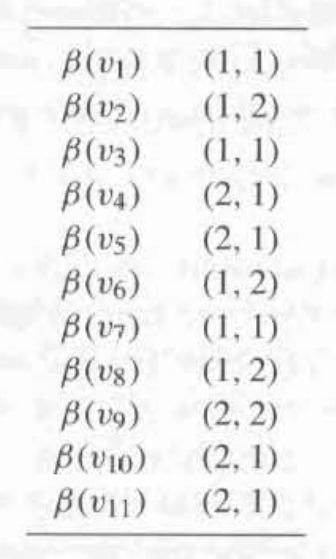
\includegraphics[width=0.18\textwidth]{tabu}
    \caption{ Tne tabulation of the binding \cite{b1}}
    \label{fig:tabu}
\end{figure}

Note that in the particular case of a non-hierarchical graph, solving the ILP problem may he far less efficient than coloring the corresponding interval graph.


\subsection{Resource sharing and binding analysis for non hierarchical graph}

Let us now consider hierarchical sequencing graphs. A simplistic approach to resource sharing is to perform it independently within each sequencing graph entity. Such an approach is overly restrictive, because it would not allow sharing resources in different entities. Therefore we consider here resource sharing across the hierarchy levels. 

Let us first restrict our attention to sequencing graphs where the hierarchy is induced by model calls. When two link vertices corresponding to different called models are not concurrent, any operation pair implementable by resources with the same type and in the different called models is compatible. Conversely, concurrency of the called models does not necessarily imply conflicts of operation pairs in the models themselves.

Consider a model a consisting of two operations: an addition followed by a multiplication. Consider also a model b consisting of two operations: a multiplication followed by an addition. Assume that the addition has l-unit delay and the multiplicalion 2-unit delay. When a model $ m1 $ has a call to model a followed by a call to model b, a and b are not concurrent and the corresponding additions and multiplications are compatible. 
Consider another model $ m2 $ with two calls to a and b that overlap in time, say with start times $ t_{a}=1 $and $ t_{b}=3 $. Then we cannot say a priori that the operations of a and b are conflicting. Indeed the multiplications are not compatible while the additions are! Both situations are shown in \ref{fig:Hierarchical_conflicts_and_compatibility}. 

Therefore the appropriate way of computing the compatibility of operations across different levels of the hierarchy is to flatten the hierarchy. Such an expansion can be done explicitly, by replacing the link vertices by the graphs of the corresponding models, or implicitly, by computing the execution intervals of each operation with respect to the source operation of the rwt model in the hierarchy. 

To determine the properties of the compatibility and conflict graphs, we need to distinguish the cases when models are called once or more than once. In both cases, model calls make the sequencing graph representation modular. In the latter case, model calls express also the sharing of the application-specific resource corresponding to the model. 


\begin{figure}[h]
    \centering
    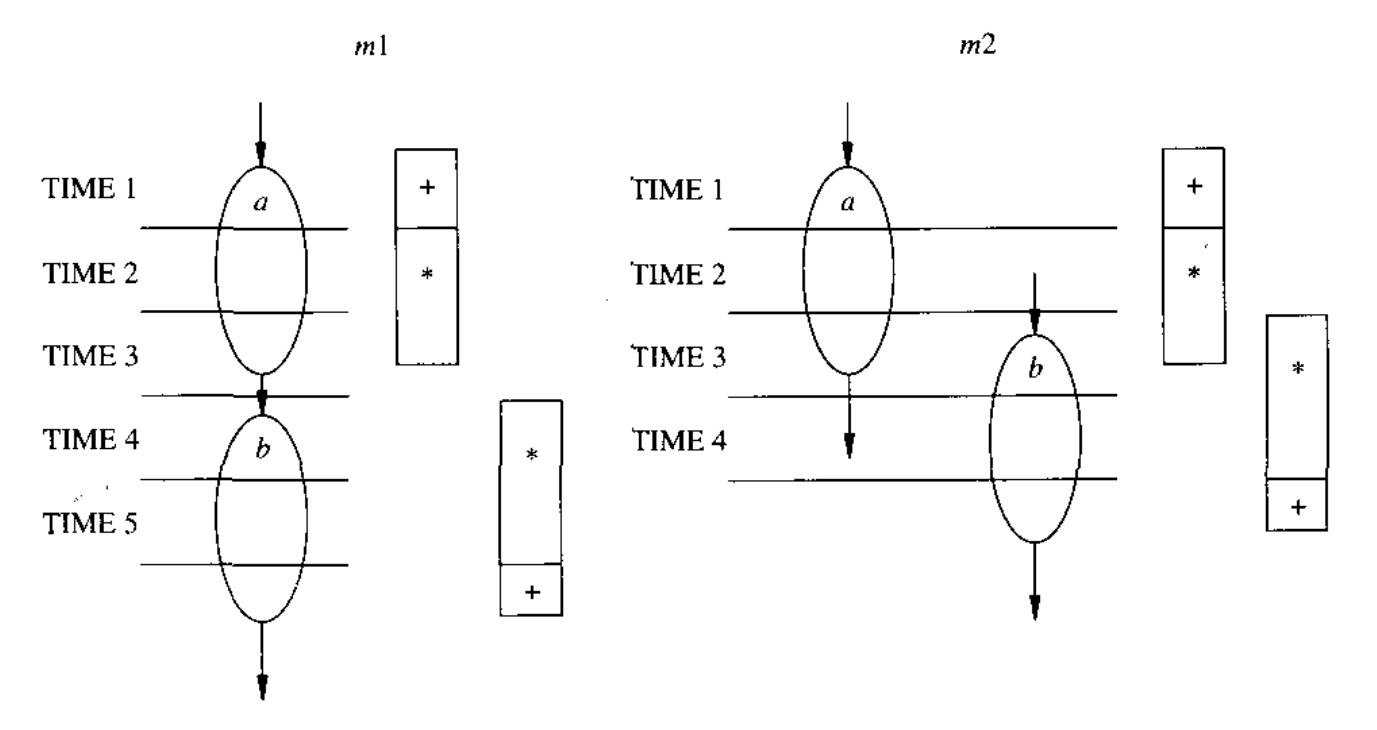
\includegraphics[width=0.5\textwidth]{Hierarchical_conflicts_and_compatibility}
    \caption{ Hierarchical conflicts and compatibility. \cite{b1}}
    \label{fig:Hierarchical_conflicts_and_compatibility}
\end{figure}


When all models are called only once, the hierarchy is only a structured representation of the data-flow information. Thus compatibility and conflict graphs have 
the special properties described in the previous section. 
Let us consider now multiple calls to s model. We question the compatibility 
or conflict of the operations in the called model with those in the calling one, and the 
properties of the corresponding graphs. 


onsider again model a consisting of two operations: an addition followed by a multiplication. By assuming that the addition has 1-unit delay and the multiplication 2-unit delay, model a has an overall delay of 3 units. Consider then model $ m3 $ with two calls to model a that are not concurrent scheduled at times 1 and 5, respectively. Assume also that model $ m3 $ has three other multiplication operations. We question the sharing of the multipliers across the hierarchy. 
A sequencing graph fragment (related to $ m3 $), the execution intervals and the conflict graph for the multiplier type are shown in Figure \ref{fig:Hierarchical_conflicts}. Note that the double call to a results in two non-contiguous execution intervals for the multiplication in a. As a result, the conflict graph is not an intersection among intervals and therefore not an interval graph. It is not even a chordal graph, as shown in Figure \ref{fig:Hierarchical_conflicts} (c).

hereas the computation of the compatibility and conflict graphs is still straightforward, the resulting graphs may no longer have special properties. Therefore their clique partitioning and vertex coloring are now intractable problems. 

\begin{figure}[h]
    \centering
    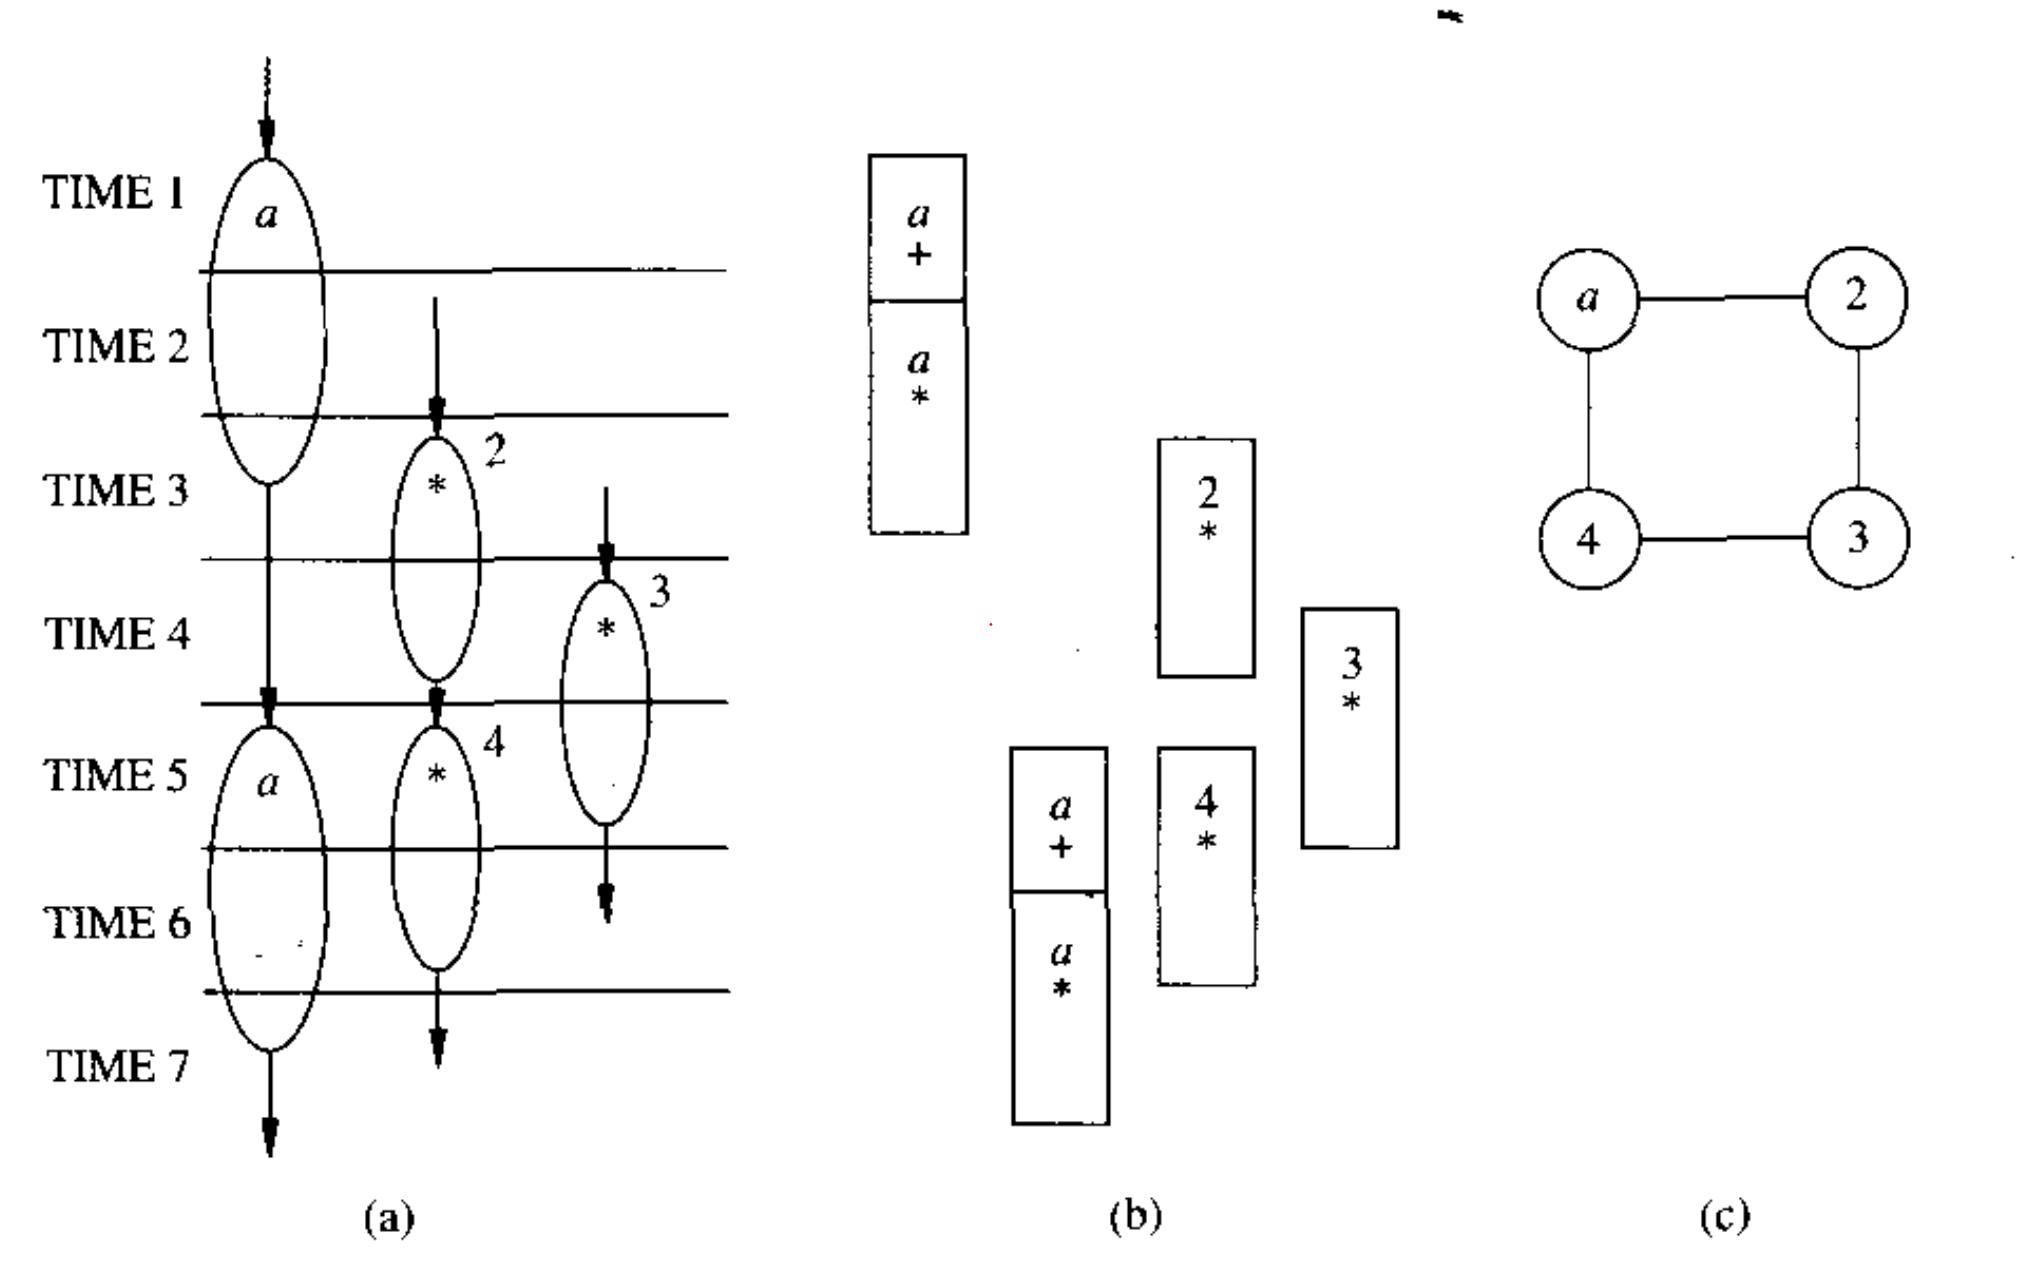
\includegraphics[width=0.5\textwidth]{Hierarchical_conflicts}
    \caption{Hierarchical conflicts. (a) Sequencing graph fragment. (b) Execution intervals. (c) Non-chordal conflict graph. \cite{b1}}
    \label{fig:Hierarchical_conflicts}
\end{figure}


The compatibility of the operations across the hierarchy can be computed in a similar way in the presence of iterative constructs that can be unrolled. Note that a resource bound to one operation in a loop corresponds to a resource bound to multiple instances of that operation when the loop is unrolled. Moreover, that resource may be bound to other operations outside the loop model. Note also that a single model call inside a loop body becomes a multiple call when the loop body is unrolled. Let us consider now branching constructs. When considering operation pairs in two alternative branching bodies, their compatibility corresponds to having the same type. The computation of the compatibility and conflict graphs can still be done by traversing the hierarchy and using Definitions  resource compatibility graph and resource conact graph. The resulting compatibility and conflict graphs may not have any special property, as shown by the following example. 

Consider the sequencing graph of Figure \ref{fig:Conditional_execution} (a). We assume that all operations take 2 time units to execute and that the start times are the following: 
$ t_{a}=1;t_{b}=3;t_{c}=t{d}=2 $. The intervals are shown in Figure \ref{fig:Conditional_execution} (b) and the conflict graph in Figure \ref{fig:Conditional_execution}(c). Note that the alternative nature of operations c and d makes them compatible and prevents a chord $ \{v_{c},v_{d}\} $to be present in the conflict graph. Hence the conflict graph is not an interval gtaph. 


\begin{figure}[h]
    \centering
    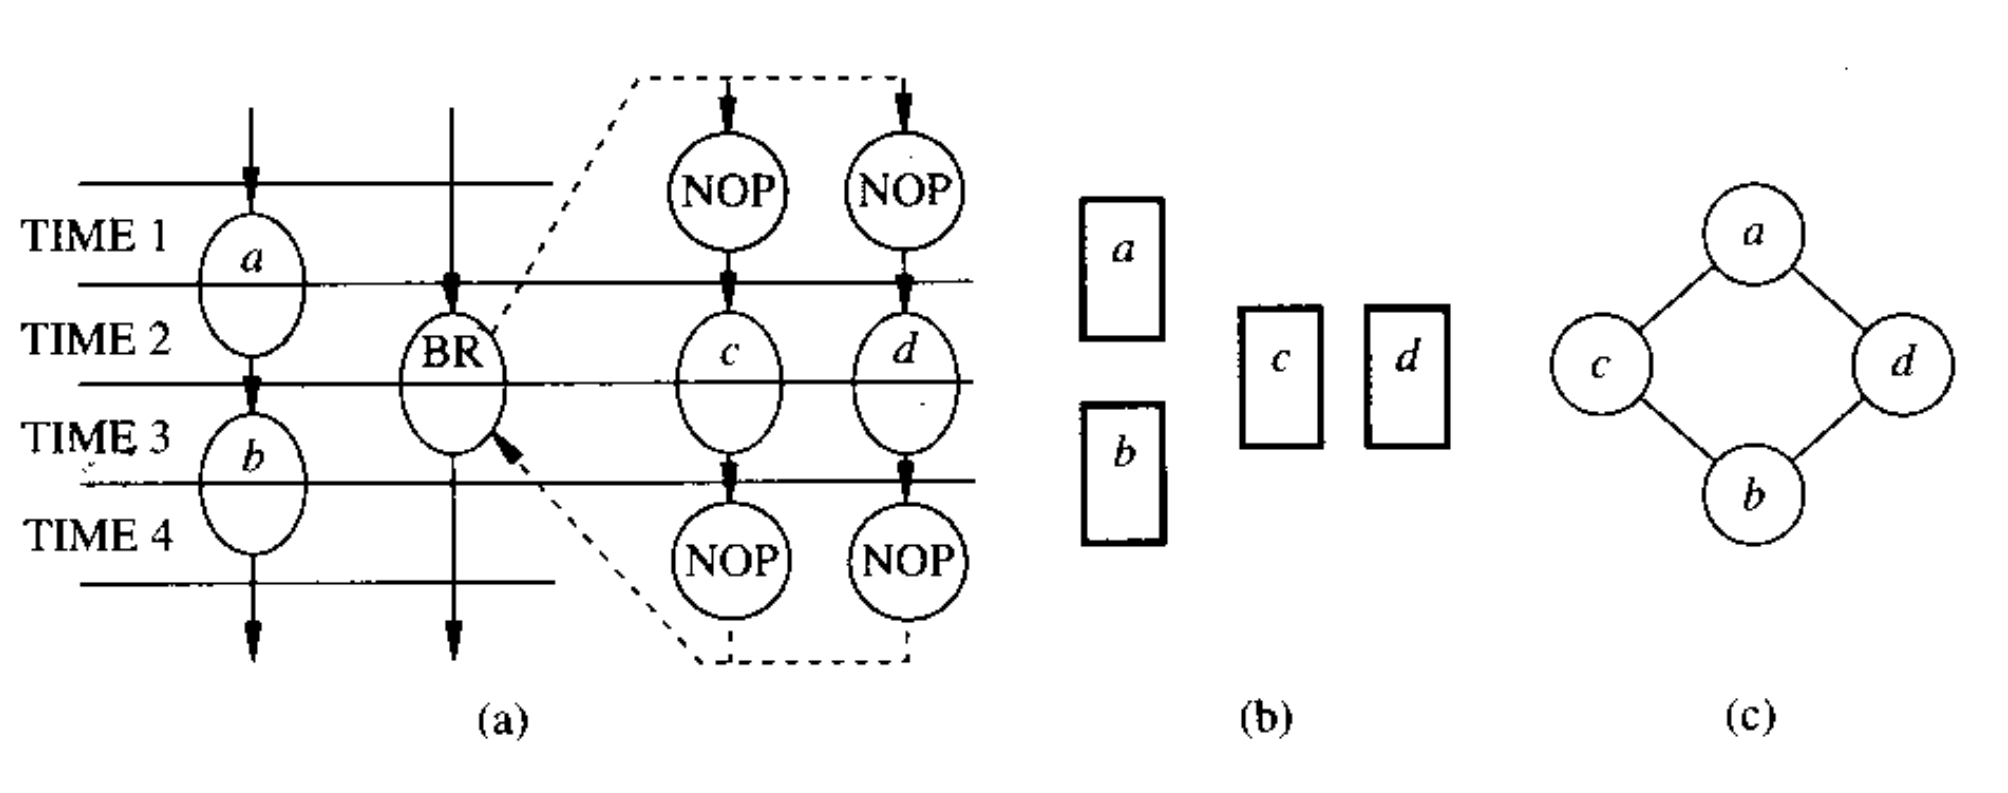
\includegraphics[width=0.5\textwidth]{Conditional_execution}
    \caption{ Conditional execution. (a) Sequencing graph fragment. (b) Execution intervals. (c) Non-chordal conflict graph \cite{b1}}
    \label{fig:Conditional_execution}
\end{figure}
\section{Non-functional Resource Sharing}


As explain before two or more operation can be bound to the same resource. Before we bond them together we need to ensure that they are \textit{compatible}. Two conditions that the operations should met in order to be \textit{compatible} :

\begin{itemize}
\item The operations is not concurrent.
\item The operations can be implemented by resources of the same type.
\end{itemize}

So, $ E+\{(v_{i},v_{j})|\tau(v_{i}=v_{j} $ and $ ((t_{i}=d_{i} \leq t_{j}) $ or $ t_{j}=d{j} \leq t_{i})),i,j=1,...,n_{ops}\}$ %


\subsection{Register Sharing}

We consider in this section those registers that hold the values of the variables. Recall that each variable has a lifetime that is the interval from its birth to its death, where 
the former is the time at which the value is generated as an output of an operation and the latter is the latest time at which the variable is referenced as an input to another operation. We assume that those variables with multiple assignments within one model are aliased, so that each variable has a single lifetime interval in the frame of reference corresponding to the sequencing graph entity where it is used. Note that the lifetimes can be data dependent, for example, due to branching and iterative constructs.

Whereas an implementation that associates a register with each variable suffices, it is obviously inefficient. Indeed, variables that are alive in different intervals or under alternative conditions can share the same register. Such variables are called compatible. The register compatibility and conflict graphs are defined analogously to the resource compatibility and conflict graphs. The problem of minimizing the number of registers can be cast in a minimum clique partitioning problem of,the compatibility graph or into a minimum coloring problem of the conflict graph. We consider now how these graphs are generated and their properties. Let us consider first non-hierarchical sequencing graphs. In this model, a conflict between two variables corresponds to a lifetime overlap. Since in this model the variable lifetimes are intervals, the conflict graph is 'an interval graph and its complement is a comparability graph. Therefore, optimum register sharing can be computed in polynomial time.

Consider just a portion of the sequencing graph of Figure \ref{Scheduled_sequencing_graph}, shown in Figure \ref{fig:Sequencing_graph_fragment}(a). There are six intermediate variables, named $ \{z_{i},i=1,2,...,6\} $, that must be stored in registers. The lifetime of three pairs of these variables is conflicting, as shown by the conflict graph in Figure \ref{fig:Sequencing_graph_fragment}(c). These variables can be implemented by two registers, which is the chromatic number of the conflict graph.


Let us now consider sequencing models of iterative bodies. In this case, some variables are alive across the iteration boundary, for example, the loop-counter variable. The cyclicity of the lifetimes is modeled accurately by circular-arc graphs that represent the intersection of arcs on a circle. We consider the full differential equation integrator. There are 7 intermediate variables $ \{z_{i},i=1,2,...,6\} $, 3 loop variables $ \{x,y,z\} $ and 3 loop invariants  $ \{a,3,dx\} $. We consider here the intermediate and loop variables and their assignment to registers. The data-flow graph is shown in Figure \ref{fig:Sequencing_graph}(a) along with the explicit annotation of the variables. The variable lifetimes are shown in Figure  \ref{fig:Sequencing_graph}((b) and are represented as arcs on a circle in Figure \ref{Variable_lifetimes_as_arcs_on_a_circle}. The corresponding circular-arc conflict graph is shown in Figure \ref{fig:Circular_arc_confliCr_graph}. Five registers suffice to store the 10 intermediate and loop variables. 

The register sharing problem can then be cast as a minimum coloring of a circular-arc graph that unfortunately is intractable. Stok [??] has shown that this problem can be transformed into a multi-commodity flow problem and then solved by a primal algorithm.

Register is used by a circuit to store values of variable. Since variable have life time it can be interval. This variable value will be use letter by other operation as an input.
\ref{fig:Sequencing_graph_fragment}
\begin{figure}[h]
    \centering
    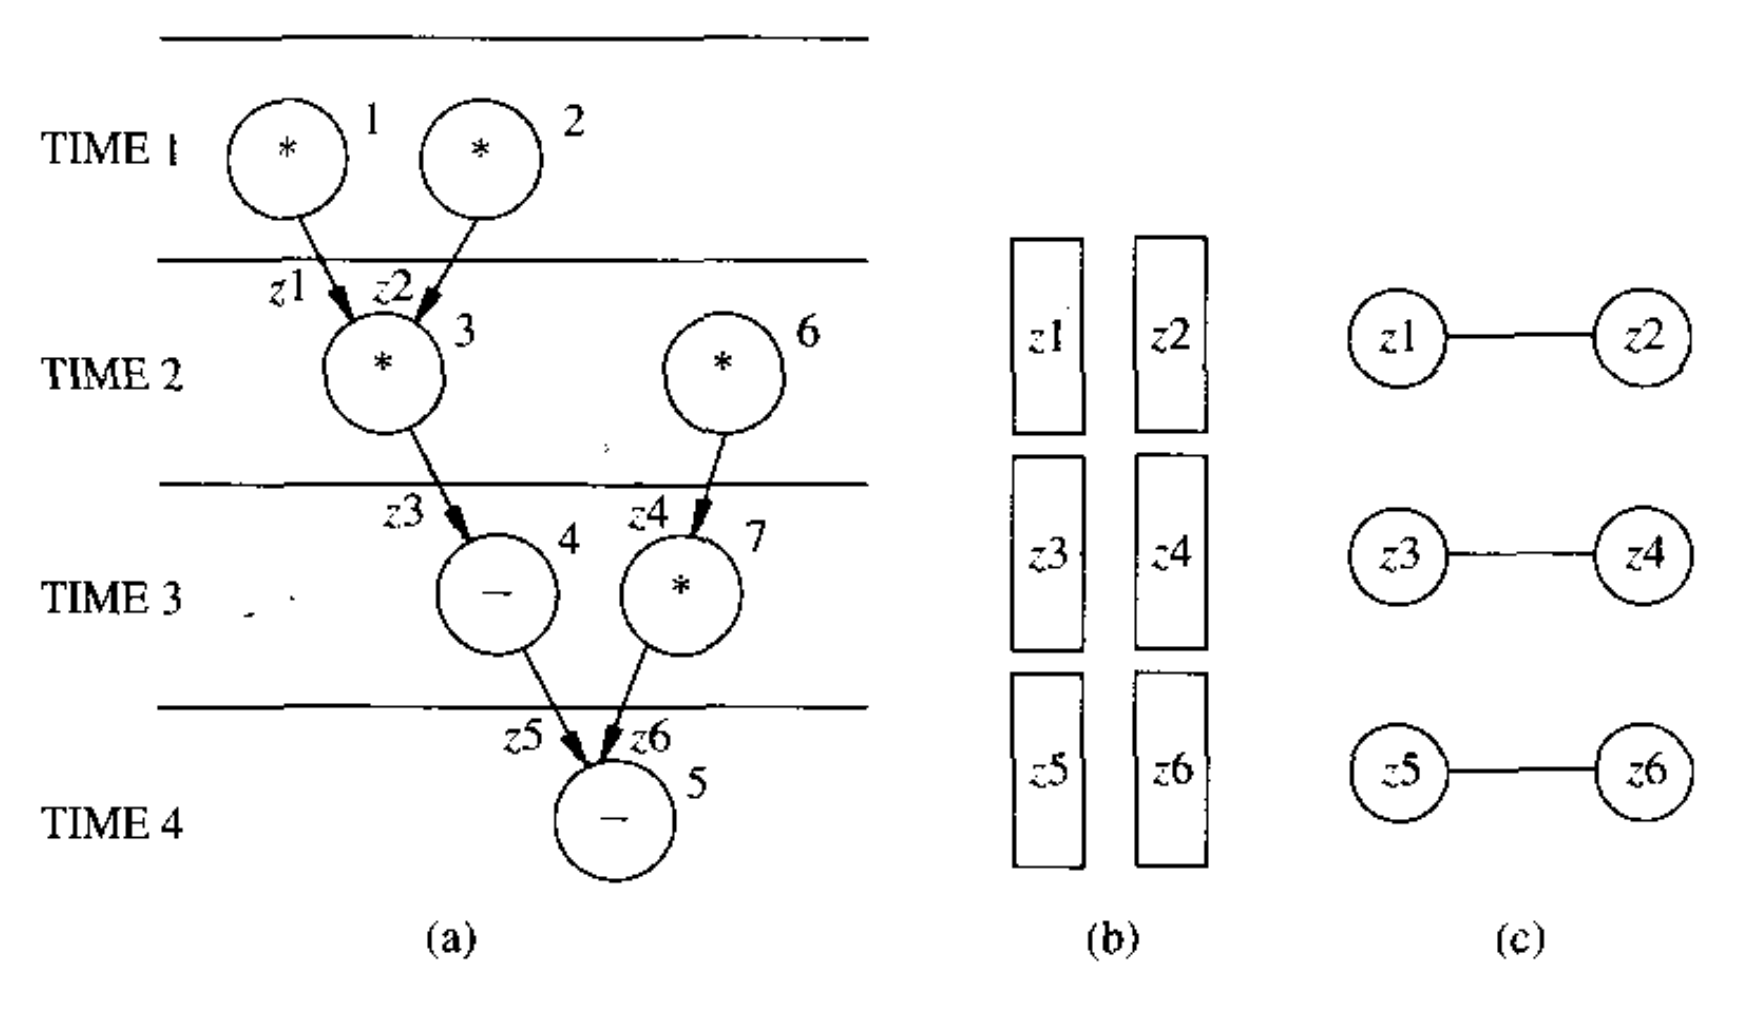
\includegraphics[width=0.5\textwidth]{Sequencing_graph_fragment}
    \caption{ a) Sequencing graph fragment. (b) Variable intervals. (c) Conflict mph \cite{b1}}
    \label{fig:Sequencing_graph_fragment}
\end{figure}

\ref{fig:Sequencing_graph}
\begin{figure}[h]
    \centering
    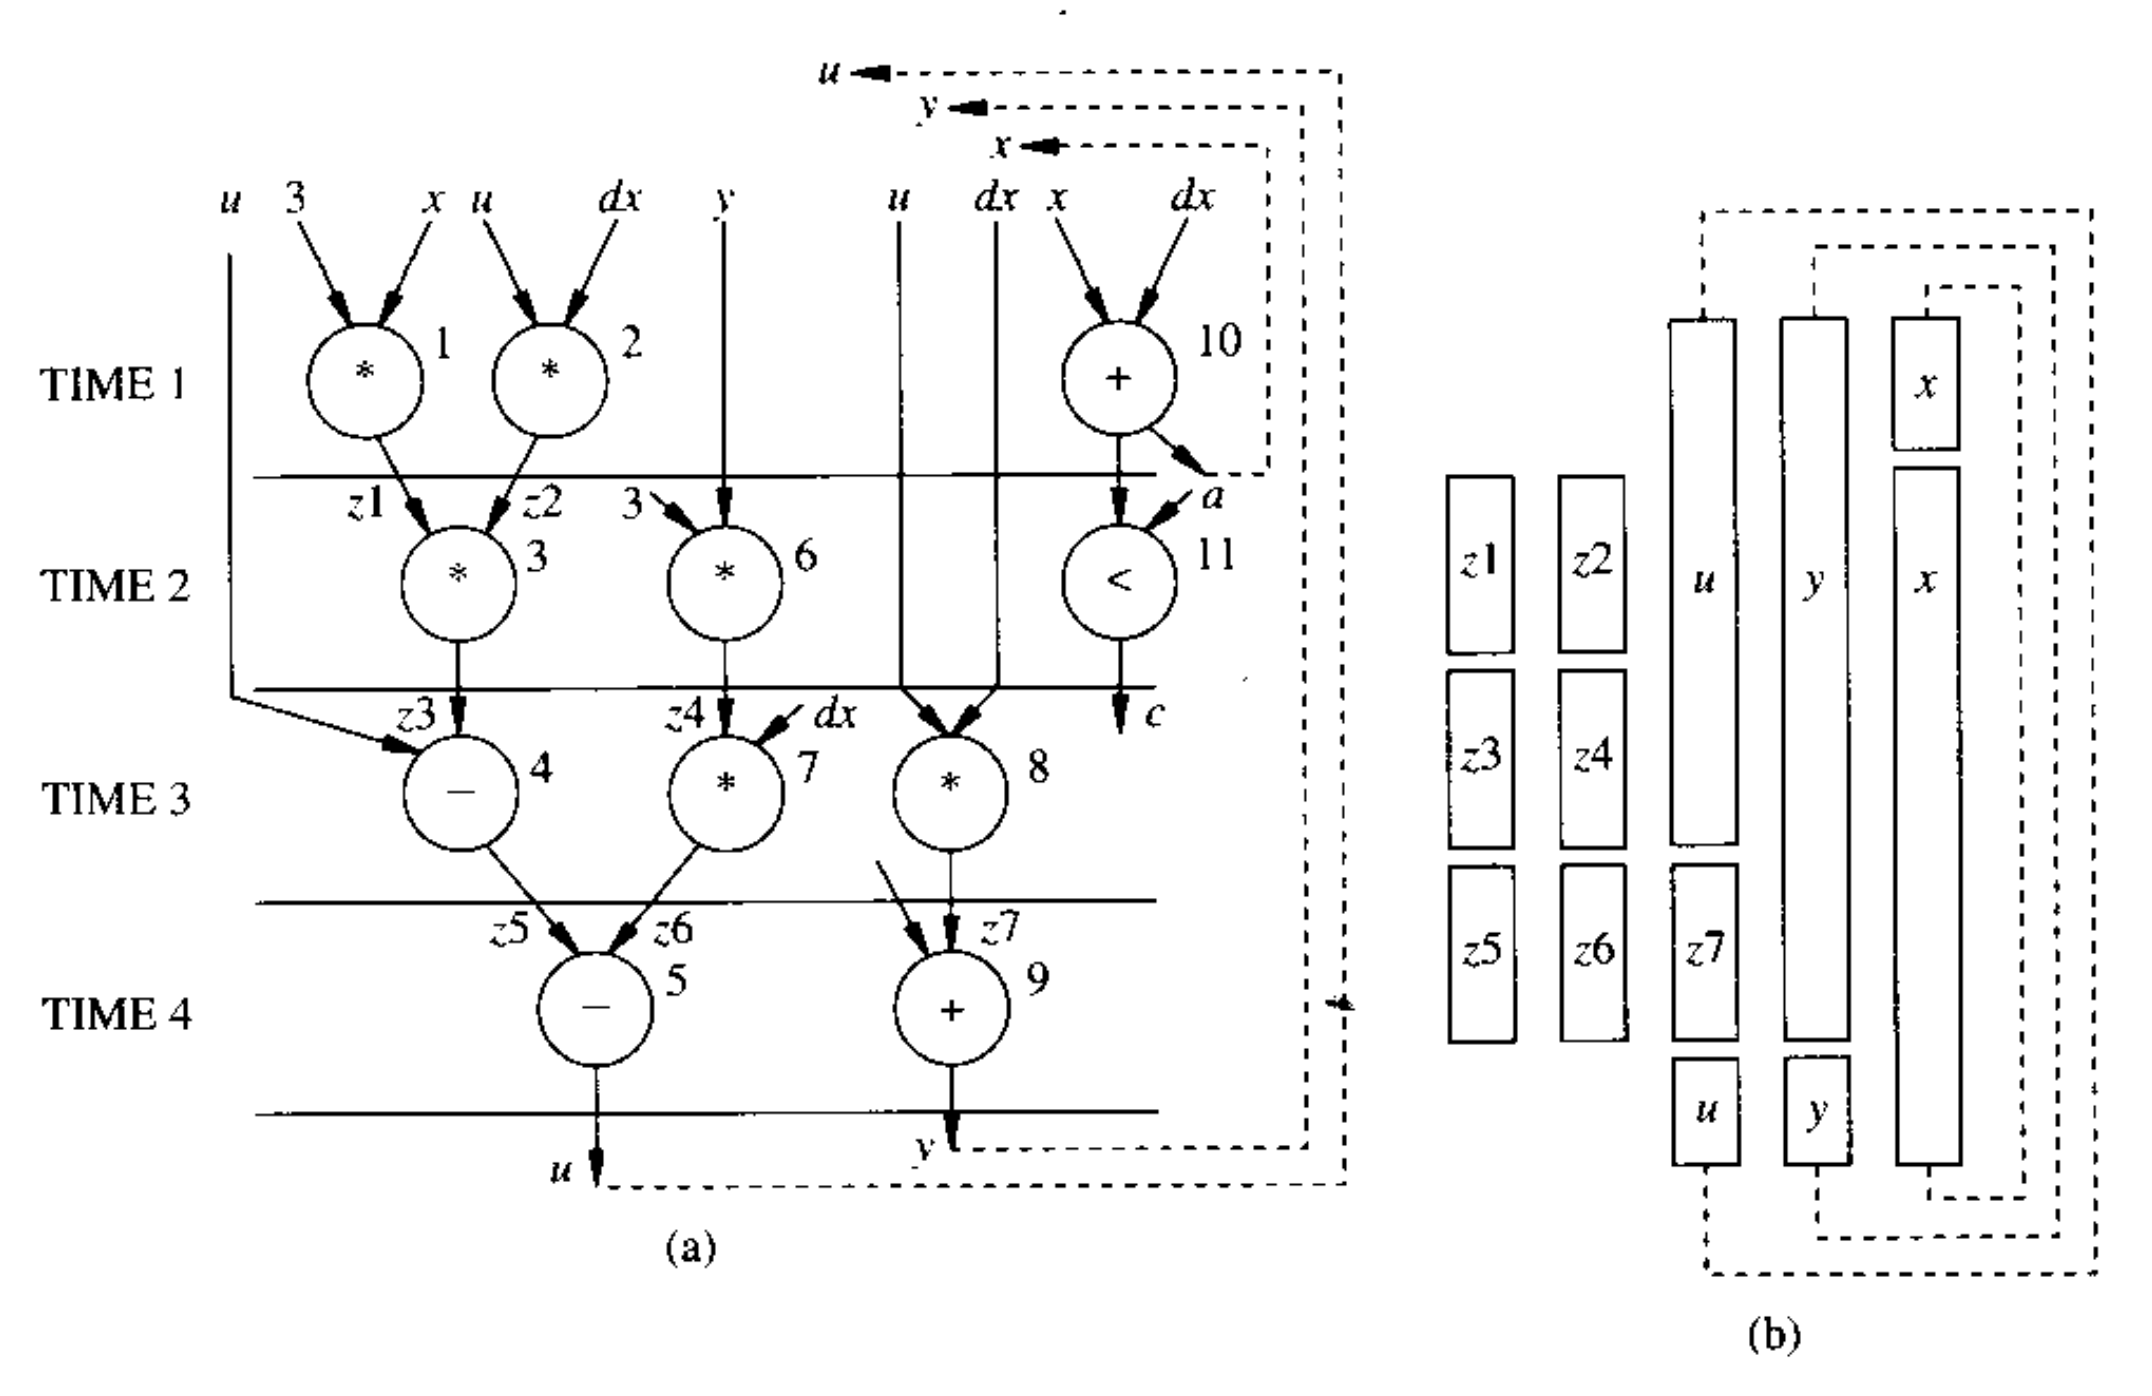
\includegraphics[width=0.5\textwidth]{Sequencing_graph}
    \caption{ (a) Sequencing graph. (b) Variable lifetimes \cite{b1}}
    \label{fig:Sequencing_graph}
\end{figure}

\ref{fig:Variable_lifetimes_as_arcs_on_a_circle}
\begin{figure}[h]
    \centering
    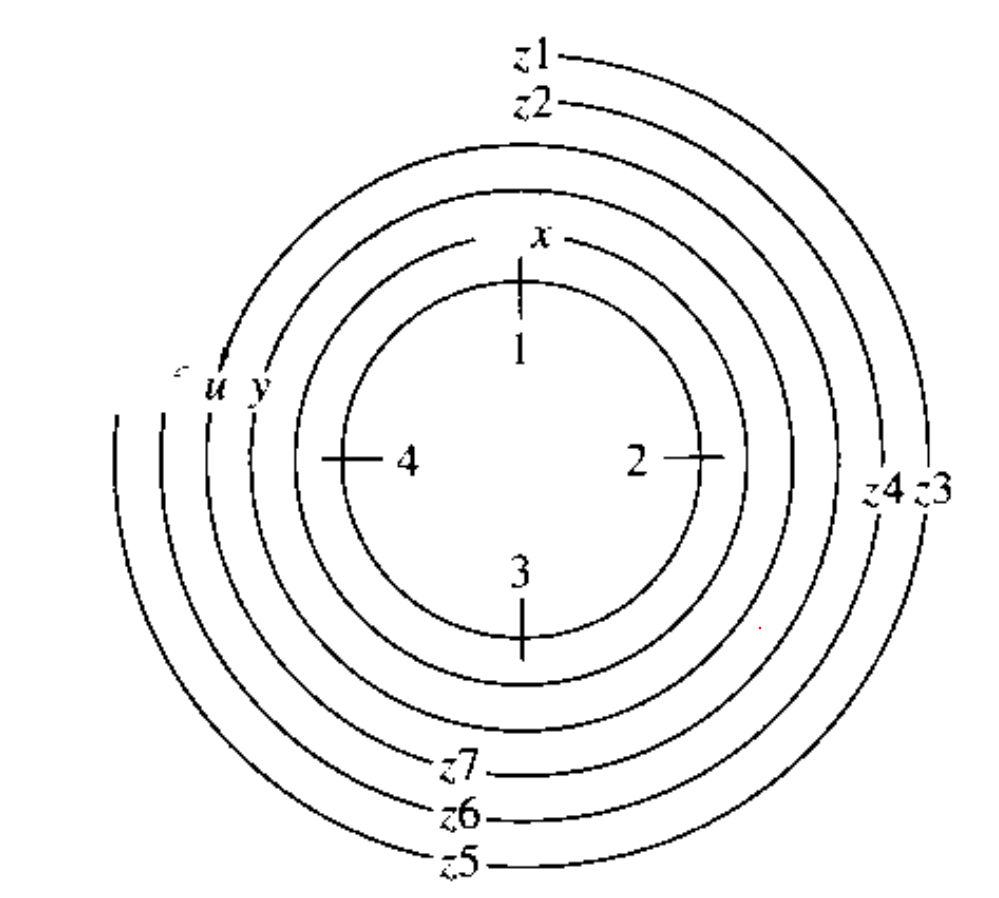
\includegraphics[width=0.4\textwidth]{Variable_lifetimes_as_arcs_on_a_circle}
    \caption{ Variable lifetimes as arcs on a circle \cite{b1}}
    \label{fig:Variable_lifetimes_as_arcs_on_a_circle}
\end{figure}

\ref{fig:Circular_arc_confliCr_graph}
\begin{figure}[h]
    \centering
    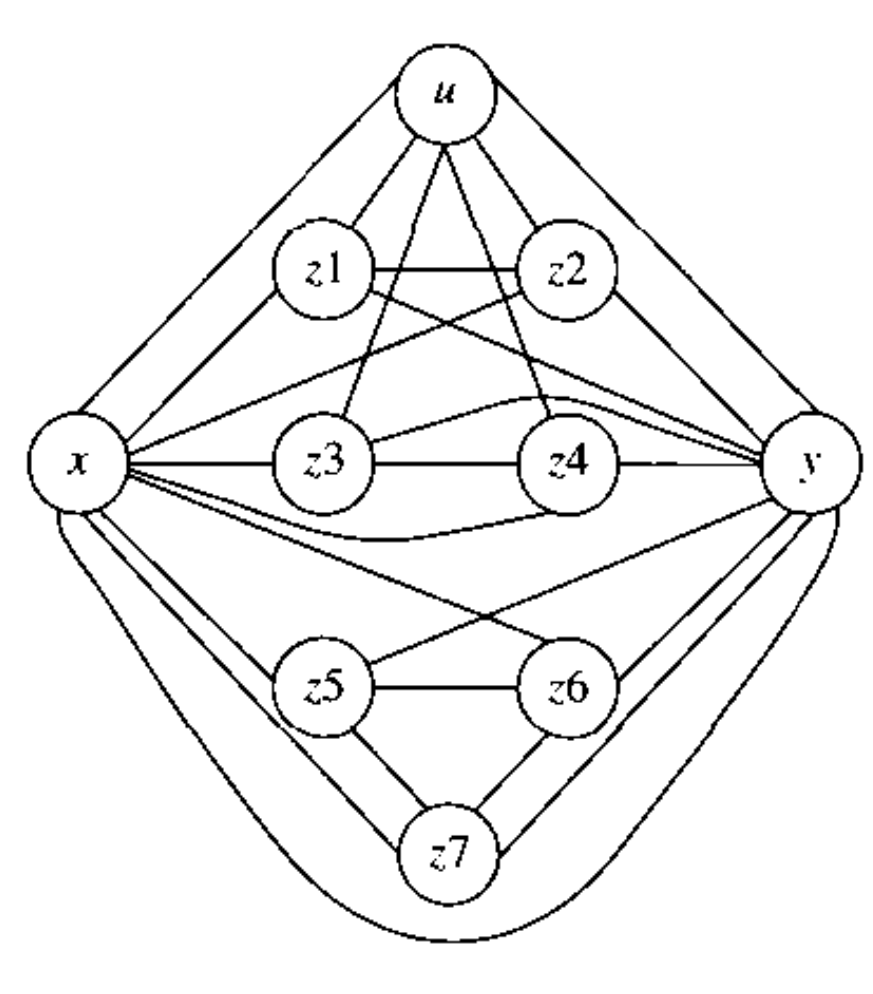
\includegraphics[width=0.4\textwidth]{Circular_arc_confliCr_graph}
    \caption{ Circular-arc conflict graph \cite{b1}}
    \label{fig:Circular_arc_confliCr_graph}
\end{figure}

The register sharing problem can be extended to cope with hierarchical models. The register compatibility and conflict graphs can be derived by traversing the hierarchy and comparing the variable lifetimes. The properties of these graphs depend on the structure of the hierarchy, as in the case of the resource compatibility and conflict graphs. In particular, interval conflict graphs can be derived from hierarchical models with only single model calls by considering the variable lifetimes with reference to the start time of the sequencing graph entity in the root model of the hierarchy. In the general case. register compatibility and conflict graphs may not have any special property, and therefore the corresponding optimum register sharing problem is intractable. 

Springer and Thomas [??] have shown that polynomial-time colorable conflict graphs can be achieved by enforcing some restrictions on the model calls and on the branch types. The register sharing problem can be formulated by ILP constraints, mutaris murandis, similarly to the resource sharing problem. 

\subsection{Multiple Memory Binding}
We consider now the problem of using multi-port memory arrays to store the values of the variables. Let us assume a memory with a ports for either read or write requiring one cycle per access. Such a memory array can be a general purpose register file common to RISC architectures. We assume the memory to be large enough to hold all data. We consider in this section non-hierarchical sequencing graphs; extensions are straightforward and similar to those presented in the previous sections. 
A first problem corresponds to computing the minimum number of ports a required to access as many variables as needed. If each variable accesses the memory always through the same port, then the problem reduces to binding variables to ports. Thus the considerations for functional resource binding can be applied to the ports, which can be seen as interface resources. 

On the other hand, if the variables can access the memory array through any port,the minimum number of ports is equal to $\underset{1\leq l \leq \lambda + 1}{\mathrm{max} \sum_{i=1}^{n_{var}} x_{il}} $ is the total number $ {n_{var}} $ of variables and X is a set of binary constants determined by scheduling, where $ x_{il} $ is 1 when the access of variable $ i,i=1,2,...,n_{var} $ is at step $ l,l=1,2,..., \lambda+1 $. In other words, the maximum number of concurrent accesses is the minimum number of ports. 
Balakrishnan et al. [??] considered the dual problem. They assumed a fixed number of ports and maximized the number of variables to be stored in the multi-port memory array, subject to the port limitation. They formulated the problem as follows. 
Let $ b \in \{0,1\}^n_{var} $  be a binary-valued vector whose entries denote whether the corresponding variable is stored in the array or not. Let $ \mathds{1} $ be a $ n_{var}  $ dimensional vector of all 1s. Then the desired variables are indicated by a solution to:

\begin{center}
$\mathds{1}^{T} b = \sum_{i=l}^{n_{var}}b_{i}$
\end{center}

\begin{equation}\label{1b}
sun_{i=l}^{n_{var}}b_{i}x_{il} \leq a \; l=1,2,..., \lambda +1 
\end{equation}

This problem can be extended easily to handle separate read and write ports and to the interconnect minimization problem [??]. 
This example is borrowed from reference [2]. Consider the following scheduled sequence of operations, which requires the storage of variables $ \{z_{i}, i =1,2,...,15\} $ 


$time-step \; 1:\; z_{3}=z_{1}+z_{2};z_{12}=z_{1}$

$time-step \; 2:\; z_{5}=z_{3}+z_{4};z_{7}=z_{3}*z_{6};z_{13}=z_{3}$

$time-step \; 3:\; z_{8}=z_{3}+z_{5};z_{9}=z_{1}*z_{7};z_{11}=z_{10}/z_{5}$

$time-step \; 4:\; z_{14}=z_{11}\wedge z_{8};z_{15}=z_{12}\vee z_{9}$

$time-step \; 5:\; z_{1}=z_{14};z_{2}=z_{15}=z_{3}$


Let us consider a memory array with a ports. Then, the problem can be represented by maximizing $  sum_{1=1}^{15} b_{i}$ under the following set of constraints: 

\begin{flushright}
$ b_{1}+b_{2}+b_{3}+b_{12}\leq a $

$ b_{3}+b_{4}+b_{5}+b_{6}+b_{7}+b_{13}\leq a $

$ b_{1}+b_{3}+b_{5}+b_{7}+b_{8}+b_{9}+b_{10}+b_{11}\leq a $

$ b_{8}+b_{9}+b_{11}+b_{12}+b_{14}+b_{15}\leq a $

$ b_{1}+b_{2}+b_{14}+b_{15}\leq a $
\end{flushright}


This problem with a one-port memory (i.e., $ a = 1 $) yields a solution where only $ \{b_{2},b_{4}b_{8} \}$are non-zero, i.e.. where only variables$ z_{2},z_{4} $ and $z_{8}$  are stored in the memory. Increasing the number of ports helps in storing more variables into the array. For example, with a two-port memory (i.e.. $ a = 2 $). variables $ z_{2},z_{4} ,z_{5},z_{10} ,z_{12}  $ and $z_{14}$ can be stored and with a three-port memory (i.e., $ a=3 $). variables$ z_{1},z_{2},z_{4} ,z_{6},z_{8},z_{10} ,z_{12},z_{13}  $ and $ z_{14} $ can be stored.

\subsection{Bus Sharing Binding}

Busses act as transfer resources that feed data to functional resources. The operation of writing a specific bus can be modeled explicitly as a vertex in the sequencing graph model. In this case, the compatible (or conflicting) data transfers may be represented by compatibility (or conflict) graphs, as in the case of functional resources. Alternatively, busses may not be explicitly described in the sequencing graph model. Their  (optimum) usage can be derived by exploiting the timing of the data transfers. Since busses have no memory, we consider only the transfers of data within each schedule step (or across two adjacent schedule steps, when we assume that the bus transfer is interleaved with the computation). 

Two problems then arise: first, to find the minimum number of busses to accommodate all (or part of) the data transfers and, second, to find the maximum number of data transfers that can be done through a given number of busses. These problems are analogous to the multi-port binding problem and can be modeled by ILP constraints. 

Consider the sequencing graph fragment of Figure \ref{fig:Sequencing_graph_fragment}(a). Let us assume that the variables of interest are $ \{z_{i},i=1,2,...,6\} $ and that busses can transfer 
the information across two adjacent steps. Let the timing scheduled data transfers be 
modeled by constants $ X=\{x_{il},i=1,2,...6;l=1,2,...,5 \}$. The values of the elements of X are all 0s. except for $ x_{11},x_{21},x_{32},x_{42},x_{53},x_{63}, $ which are 1s. Then Equation \ref{1b} yields:

$ b_{1}+b_{2} < a $

$ b_{3}+b_{4} < a $

$ b_{5}+b_{6} < a $


Let us consider first the case of $ a = 1 $ bus. Then at most three variables can be transferred 
on the bus, for example $ \{z_{1},z_{3},z_{5}\} $. With a = 2 busses all variables can be transferred. 

\subsection{Multiplexer}

\subsubsection{Unconstrained minimum-area binding }
\subsubsection{Example}
consider:

$ n $ add operation

$ a $ adders

$ area_{mux} $ area off Multiplexer


$ area(area_{add}+area_{mux})\approx a(area_{add}- area_{mux}^{\bigtriangleup})+n \cdot area_{mux}^{\bigtriangleup}  $

$ area\approx a\cdot (area_{add}+(\frac{n}{a}-1)) \cdot area_{mux}^{\bigtriangleup} $

$  area=a\cdot (area_a{add}-area_{mux}^{\bigtriangleup})+n\cdot area_{mux}^{\bigtriangleup}$


$area_{mux} = (i-1)\cdot area_{mux}^{\bigtriangleup} $

$=-area_{mux}^{\bigtriangleup} + i \cdot area_{mux}^{\bigtriangleup}  $

$=area_{M}^{0} + sum_{j=1}{i} area_{M}^{j}$

$ area_{M}^{0} = -areaarea_{mux}^{\bigtriangleup} $

$ area_{M}^{j}=area_{mux}^{\bigtriangleup} $

%$ area_{mux}^{\bigtriangleup} $

%$area_{mux} \approx area_{mux}^{\bigtriangleup}(i-1) $


%$ area_{add} > area_{mux}^{\bigtriangleup} $


\ref{fig:Comparibility_graph_mux}
\begin{figure}[h]
    \centering
    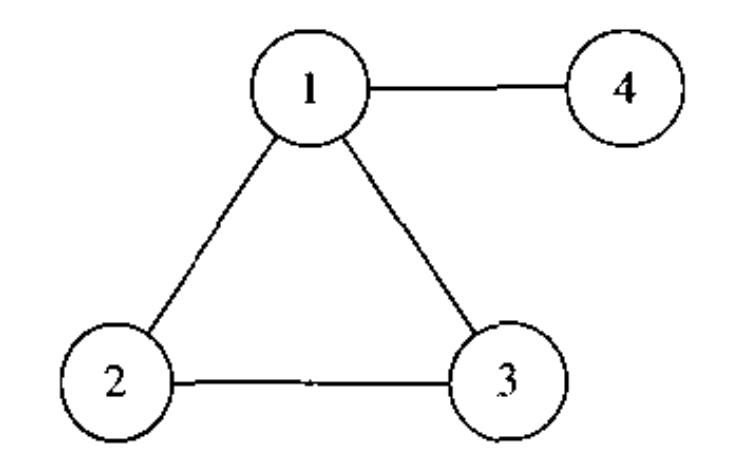
\includegraphics[width=0.3\textwidth]{Comparibility_graph_mux}
    \caption{ Compatibility graph \cite{b1}}
    \label{fig:Comparibility_graph_mux}
\end{figure}

\ref{fig:Comparibility_graph_mux_2}
\begin{figure}[h]
    \centering
    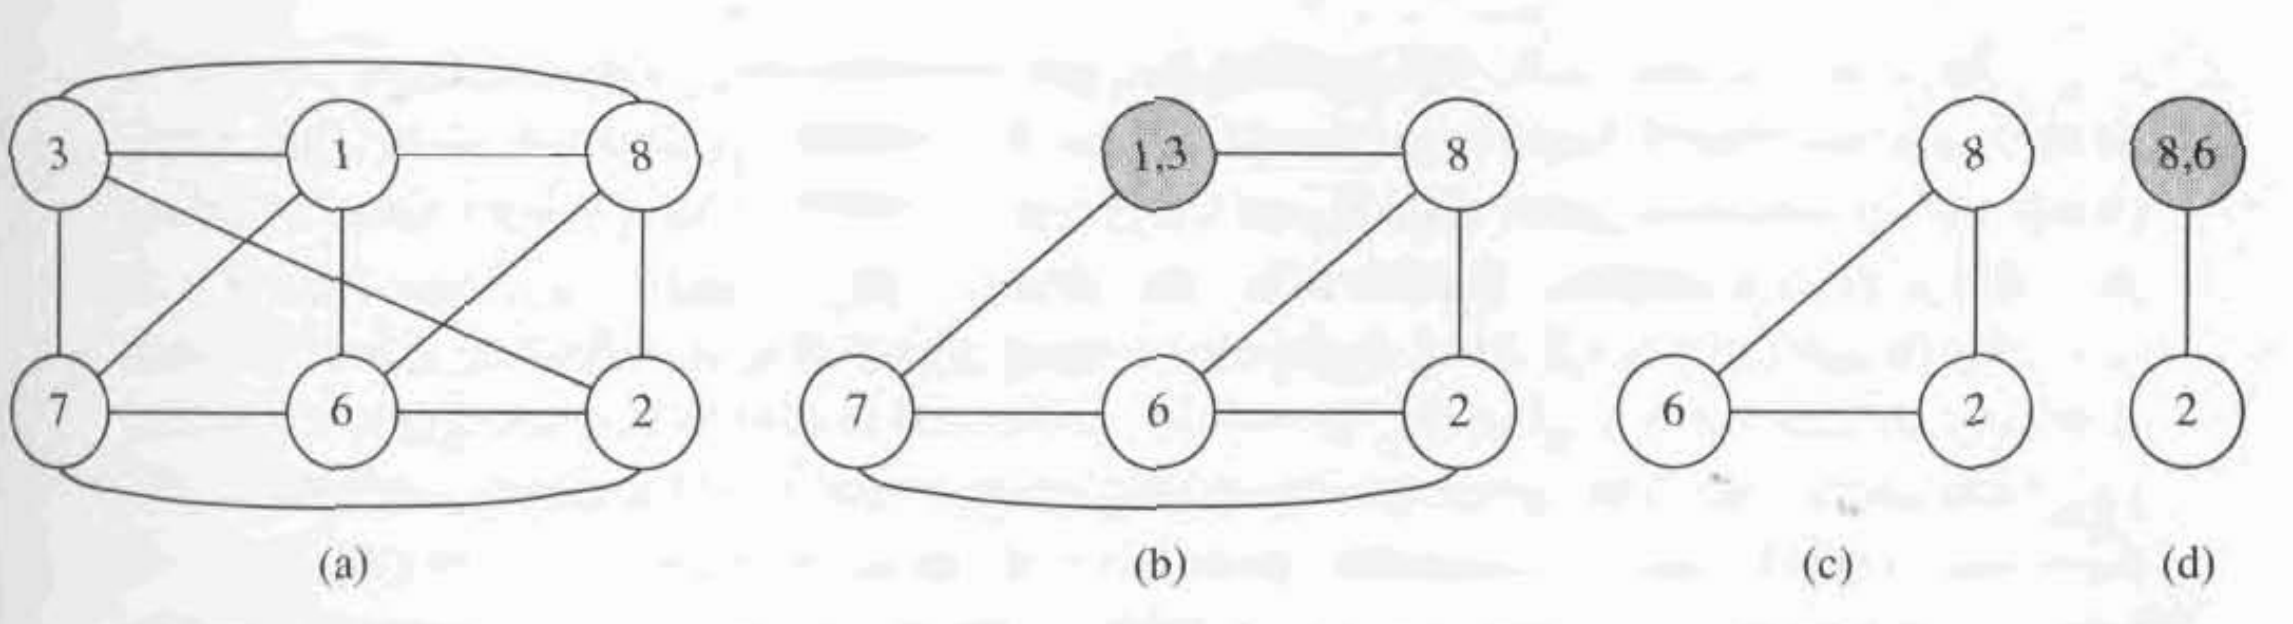
\includegraphics[width=0.5\textwidth]{Comparibility_graph_mux_2}
    \caption{ (a) Compatibility graph for the multiplier type. (b) Reduced compatibility graph with clique seed. (c) Fragment of compatibility graph after one clique has heen removed. (d) Reduced fragment with clique seed. \cite{b1}}
    \label{fig:Comparibility_graph_mux_2}
\end{figure}





%abstract
%
%Introduction
%	Sharing and binding
%
%Basic concept
%	graph
%	resources 
%	constraint
%
%problem+approach
%
%Resource dominated circuit
%
%General circuit



\section{Conclusion}

\section*{Acknowledgment}
I would like to express my very great appreciation to Dr Achim Rettberg for his valuable and constructive suggestions during the planning and development of this research work. His willingness to give his time so generously has been very much appreciated.

\begin{thebibliography}{00}
\bibitem{b1} G. D. Micheli, Synthesis and optimization of digital circuits. New York: McGraw-Hill, 1994.
\bibitem{b2} Shilpa, K. and Lakshminarayana, C and Singh, Manoj. (2019). Optimal Resource Allocation and Binding in High-Level Synthesis Using Nature-Inspired Computation. 10.1007/978-981-13-5802-9-95.  
\end{thebibliography}


\end{document}
